%
% system_overview.tex
%
% Copyright (C) 2021 by SpaceLab.
%
% Battery Module 4C Documentation
%
% This work is licensed under the Creative Commons Attribution-ShareAlike 4.0
% International License. To view a copy of this license,
% visit http://creativecommons.org/licenses/by-sa/4.0/.
%

%
% \brief System Overview chapter.
%
% \author Gabriel Mariano Marcelino <gabriel.mm8@gmail.com>
% \author André Martins Pio de Mattos <andrempmattos@gmail.com>
% \author Yan Castro de Azeredo <yan.ufsceel@gmail.com>
%
% \institution Universidade Federal de Santa Catarina (UFSC)
%
% \version 0.1.0
%
% \date 2020/01/22
%

\chapter{System Overview} \label{ch:system-overview}

The board is a 2 layer 1.6mm thick PCB with FR-4 dieletric. The board has PC104 through hole pads for a connector, however for the v0.1 of the project the interface is not used for any signals, power or mechanical fitting.
The power from the batteries are conducted by a pin header making a board-to-board connection to the EPS2 module. The power for the heaters actuation and the temperature sensor (RTD\nomenclature{RTD}{\textit{Resistance Temperature Detectors.}}) measurements are brought through PicoBlade connectors via external cables to the EPS2.
The \autoref{fig:block-diagram} presents the simple block diagram of the module.

\section{Block Diagram}

\begin{figure}[!ht]
    \begin{center}
        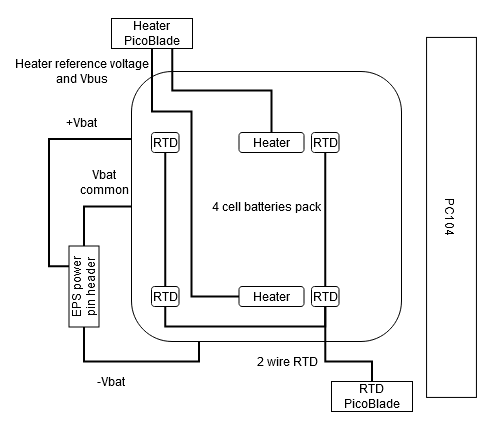
\includegraphics[width=0.65\textwidth]{figures/bat4c_block_diagram}
        \caption{Battery Module 4C Block Diagram.}
        \label{fig:block-diagram}
    \end{center}
\end{figure}